% \documentclass[10pt]{article}
\documentclass[conference, a4paper]{IEEEtran}
\usepackage[british]{babel}
\usepackage[utf8]{inputenc}
\usepackage{csquotes} % needed for babel
\usepackage{etoolbox} % alter default commands
%\usepackage{multirow} % Allows for multiple rows
%\usepackage{multicol} % Allows for multiple columns
%\usepackage[dvips,letterpaper,margin=1.5cm,bottom=2.5cm,top=2.5cm]{geometry}
\usepackage{url}
\bibliographystyle{IEEEtran.bst}
\usepackage{rotating}
\usepackage{makecell}
\usepackage{adjustbox}
\usepackage{tabularx}
\usepackage{lmodern}
\renewcommand{\familydefault}{\sfdefault}

% Images preamble
\usepackage{graphicx}% Import graphics
\usepackage{wrapfig} % Wrap figure around text
\usepackage{tikz} % Draw shapes
\usetikzlibrary{positioning,chains}
\usepackage{float}% Correcting the positioning of images

% Table preamble
\usepackage{geometry}
\usepackage{xtab, array, booktabs, caption, ragged2e, lscape, threeparttablex}
\makeatletter
\def\ifGm@preamble#1{\@firstofone}
\appto\restoregeometry{%
  \pdfpagewidth=\paperwidth
  \pdfpageheight=\paperheight}
\apptocmd\newgeometry{%
  \pdfpagewidth=\paperwidth
  \pdfpageheight=\paperheight}{}{}
\makeatother

\title{Automatic Detection of Mind Wandering from Multimodal Datastreams: A Survey of State-of-the-art Methods}
\author{\IEEEauthorblockN{Murtadha Al Nahadi, Robin Faber, Justin de Haan, Wessel Turk}
\IEEEauthorblockA{Delft University of Technology\\
Delft, Netherlands\\
\{M.AlNahadi, R.J.Faber, J.C.deHaan, W.R.A.Turk\}@student.tudelft.nl}}
\date{March 2019}

\begin{document}
\maketitle

\begin{abstract}
    Objective: The aim is to give a clear and structured overview of the current state of the art of automatic detection of mind wandering from multimodal datastreams.

Method: This survey is a literature study done by finding and analyzing existing publications regarding the subject. From an initial 129 publications, a total of 18 were selected to be analyzed in our study.

Results: All evaluated studies are summarized in Table \ref{tab:data}, including the performance of the study if applicable.

Conclusion: Considering how new the automatic detection of mind wandering is as a research subject, there have been a lot of studies using different detection technologies with good success. This shows that there is good opportunities for real-world applications of these technologies that can help prevent mind wandering, for example to prevent mind wandering while driving or attending a lecture.
\end{abstract}
    
\begin{IEEEkeywords}
    Mind wandering, literature review, machine learning, automatic detection, attentional state estimation. 
\end{IEEEkeywords}


\section{Introduction}
Mind wandering (MW) is a phenomenon where the thoughts of a person shift from task-related to task-unrelated for a certain period of time.
Every person has probably experienced it at some point and it can come paired with inefficiency and distraction. 
In situations where attention is needed, such as driving, it is important that the mind wanders as little as possible so people can focus on the task at hand. 
Recent research has clearly shown that inattention when driving has an indisputable impact on road safety \cite{berthie2015restless}. 
It is clear that automated detection and prevention of mind wandering in such settings could be a good solution to the problem. 

This study aims to identify possible challenges in the field of automatic detection of MW in order to further develop it or to be used as a starting point for people who wish to do research and want an overview of the possibilities and what has been done already. This goal is accomplished by giving a structured overview of the state-of-the-art methods in the field and reasoning about the broader context of these studies.

We investigated the following aspects of existing research:
In which tasks is the automatic detection of MW being utilized? Which modalities are used? Which sensors are used for recording these modalities and which features are extracted from them? How is MW being reported by the participants? Which machine learning (ML) algorithms are used to train the model and what performance is achieved by the model? In which environment has the data been collected and has this data been made publicly available? 
 

\section{Method}

In order to identify all articles that may be deemed relevant, a highly systematic approach was used that can be broken down into six steps (Fig. \ref{fig:prisma}).

First, 10 articles were hand-picked that were identified as relevant for our goal. These hand-picked articles served as a baseline for the upcoming search of online libraries.
A systematic search on Scopus and Web of Science was performed to identify all articles aimed at the detection of mind wandering. The retrieved articles were checked on relevancy and completeness.
An indication of the completeness of the search terms used was obtained by comparing the results of the online libraries with the baseline. 
The used search terms were tweaked by making them broader when the results contained a low number of articles and few baseline articles and made narrower when there were many irrelevant articles retrieved.
A logbook of the used search terms can be found in Appendix A.
As a result of this first step, an initial list of 125 articles was obtained.

\begin{figure}
  \resizebox{\columnwidth}{!}{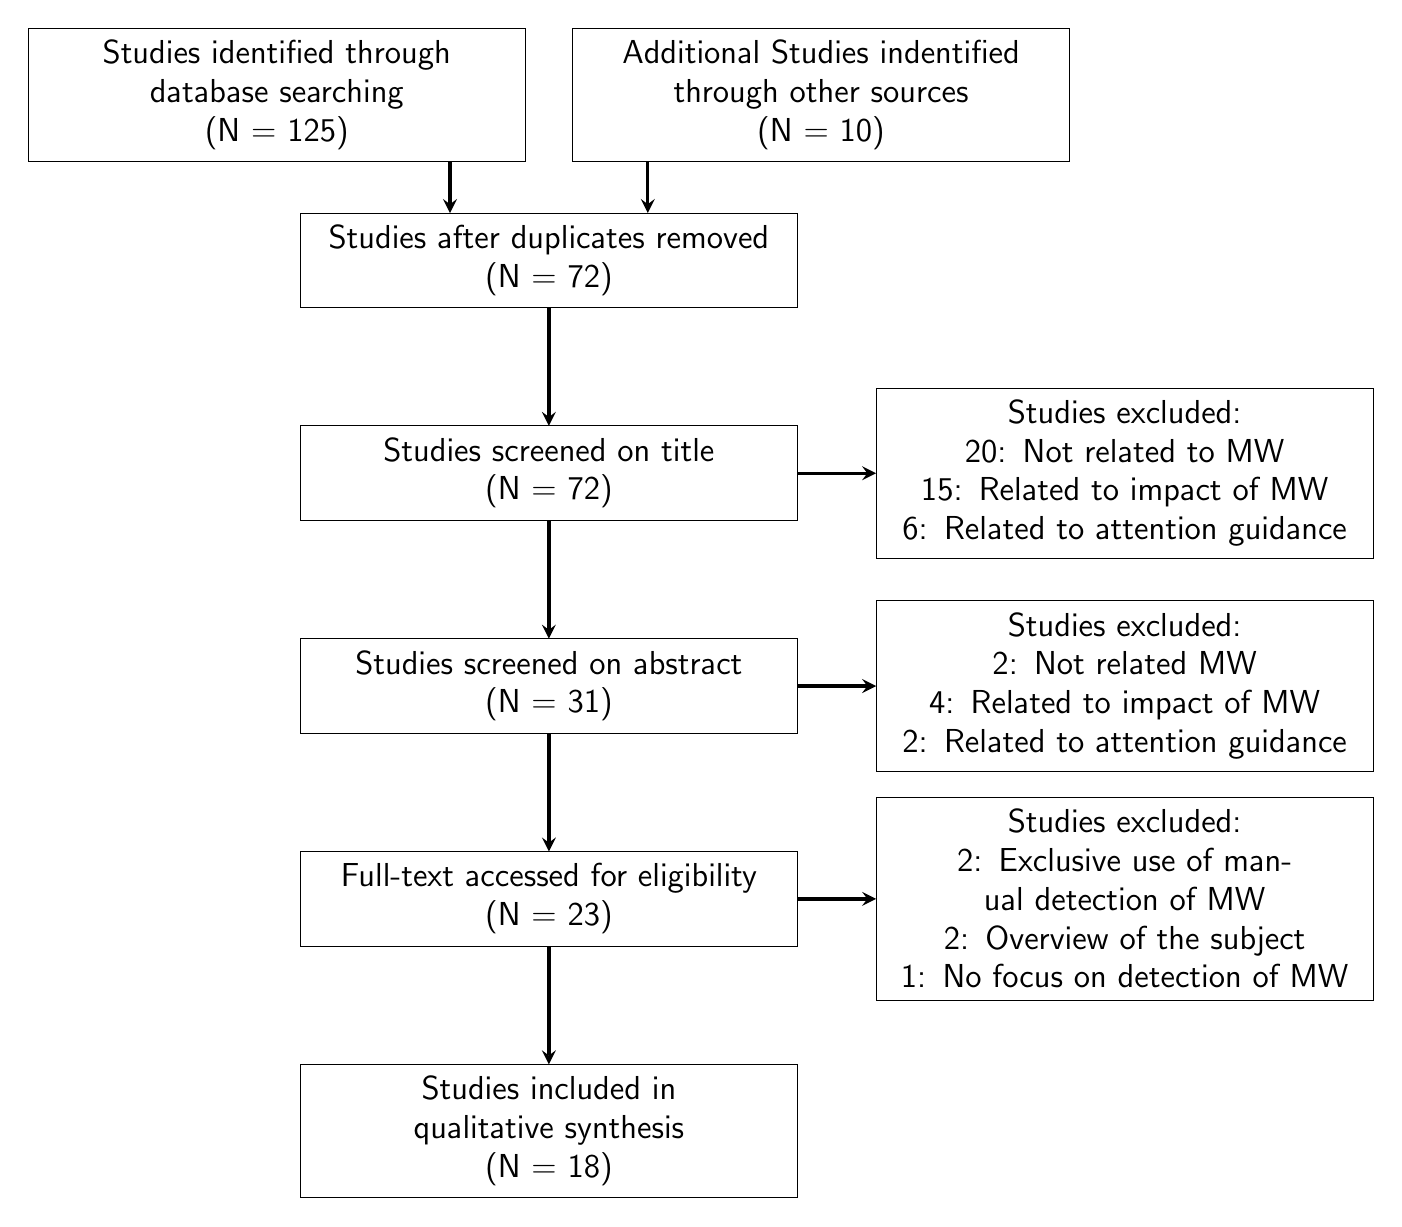
\begin{tikzpicture}[
    node distance=15mm and 10mm,
    start chain=going below,
 mynode/.style = {
        draw, rectangle, align=center, text width=60mm,
        font=\large, inner sep=1ex, outer sep=0pt,
        on chain},
mylabel/.style = {
        draw, rectangle, align=center, rounded corners, 
        font=\small\bfseries, inner sep=2ex, outer sep=0pt,
        fill=cyan!30, minimum height=35mm,
        on chain},
every join/.style = arrow,
     arrow/.style = {very thick,-stealth}
                    ] 
\coordinate (tc);
% the title
%\node[above=of tc,font=\bfseries] {PRISMA 2009 Flow Diagram};
% the nodes at the top
\node (n1a) [mynode, left=of tc, xshift=7mm]    {Studies identified through
                                        database searching\\
                                        (N = 125)};
\node (n1b) [mynode,right=of tc, xshift=-7mm]    {Additional Studies indentified\\
                                        through other sources\\
                                        (N = 10)};
    % the chain in the center
\node (n2)  [mynode, below=of tc]   {Studies after duplicates removed\\
                                        (N = 72)};
\node (n3)  [mynode,join]   {Studies screened on title\\
                                (N = 72)};
\node (n4)  [mynode,join]   {Studies screened on abstract\\
                                (N = 31)};
\node (n5)  [mynode,join]   {Full-text accessed for eligibility\\
                                (N = 23)};
\node (n6)  [mynode,join]   {Studies included in qualitative synthesis\\
                                (N = 18)};
% \node (n7)  [mynode,join]   {\# of studies included in quantitative sysntesis\\
%                                (meta-analysis)};
% the branches to the right
\node (n3r) [mynode,right=of n3]    {Studies excluded:\\
                                        20: Not related to MW\\
                                        15: Related to impact of MW\\
                                        6: Related to attention guidance
                                        };
\node (n4r) [mynode,right=of n4]    {Studies excluded:\\
                                    2: Not related MW\\
                                    4: Related to impact of MW\\
                                    2: Related to attention guidance
                                    
                                        };
\node (n5r) [mynode,right=of n5]    {Studies excluded:\\
                                        2: Exclusive use of manual detection of MW\\
                                        2: Overview of the subject\\
                                        1: No focus on detection of MW};
% lines not included in join                                        
\draw[arrow] ([xshift=+22mm] n1a.south) coordinate (a)
                                       -- (a |- n2.north);
\draw[arrow] ([xshift=-22mm] n1b.south) coordinate (b)
                                       -- (b |- n2.north);
\draw[arrow] (n3) -- (n3r);
\draw[arrow] (n4) -- (n4r);
\draw[arrow] (n5) -- (n5r);
% the labels on the left
%    \begin{scope}[node distance=5mm]
%\node[mylabel,below left=-3mm and 5mm of n1a.north west]
%                {\rotatebox{90}{Identification}};
%\node[mylabel, minimum height=40mm]  {\rotatebox{90}{Screening}};
%\node[mylabel]  {\rotatebox{90}{Eligibility}};
%\node[mylabel]  {\rotatebox{90}{Included}};
%    \end{scope}
\end{tikzpicture}}
\caption{Flow Diagram outlining the screening process}
\label{fig:prisma}
\end{figure}

Second, all duplicates obtained from the different libraries were removed, leaving 72 articles.

Third, from this point onward, all remaining articles were divided into two stacks. Each stack was reviewed individually by two team members.
The articles were screened on their title and were excluded if team members reached consensus on their irrelevancy. 
This resulted in three exclusion criteria:
\begin{enumerate}
    \item \textbf{Not related to Mind Wandering}, e.g. \cite{ISI:000432512400017}, focuses on different formats to present lecture material and is therefore excluded.
    \item \textbf{Related to the impact of Mind Wandering}, e.g. \cite{Albert2018LinkingDrivers}, concludes that mind wandering while driving leads to dangerous behaviour behind the wheel and is thus excluded.
    \item \textbf{Related to attention guidance}, e.g. \cite{Xiao2018ClassroomMechanism}, explores gamification to restore students' attention level in classroom teaching and is thus excluded.
  \end{enumerate}
In case of uncertainty, articles were included to be screened on abstract. This step narrowed the list of articles down to 31.

Fourth, Eight articles were excluded while screening on abstract, leaving 23 articles remaining. 
The excluded articles fit the earlier defined exclusion criteria but looked interesting based on their title.

Fifth, every remaining article was accessed and screened on their full-text. This included reading the methodology, results, conclusion and inspecting their figures and tables.
Two papers were excluded because they give an overview of the field, rather than explaining (new) methods of detecting mind wandering. 
Another two articles were excluded because they use manual reporting exclusively.

At last, one article was excluded because it describes a system that uses third-party solutions to detect mind wandering. The focus of this article lays on implementing this system in a learning environment, rather than on combining/improving detection methods for mind wandering.
In conclusion, a total of 18 articles are left to review.

Finally, the articles were carefully studied, extracting data of the methods used to detect mind wandering and storing these data in a table. This table is then further analyzed.


\section{Results}
A total of 18 studies were included in our review, a summary of the studies is shown in Table \ref{tab:data}. For each study the following was defined: the task people had to perform, the modalities used, the extracted features, used equipment, how people reported MW, used machine learning (ML) algorithms and the performance of the developed classifier. In the following sections, the contents and relevance of the columns from Table \ref{tab:data} will be discussed.

\newgeometry{hmargin=1.4cm,vmargin=1.0cm,landscape}
\onecolumn % use the full width of the page
% header and footer information
\topcaption{Detection methods for mind wandering} \label{tab:data}
\tablefirsthead{\toprule}
% the contents of each repeating tabular head. 
\tablehead{\multicolumn{2}{l}{Table \ref{tab:data}}{continued from previous page}\\
        \toprule
        Reference & Task & Modalities used & Sensors Used & Features Extracted \footnotemark[1] & Reporting MW \footnotemark[2] & ML algorithm(s) & Performance & Notes\\
        \midrule}
% Tabular head of last page of the table 
\tablelasthead{\multicolumn{2}{l}{Table \ref{tab:data}} concluded from previous page\\
        \toprule
        Reference & Task & Modalities used & Sensors Used & Features Extracted \footnotemark[1] & Reporting MW \footnotemark[2] & ML algorithm(s) & Performance & Notes\\
        \midrule}
\tabletail{\hline\multicolumn{9}{r}{{Continued on next page}} \\ \bottomrule}

% Start of Table
\begin{ThreePartTable}
\small % change font size to small. If not used change column size performance  24 -> 27mm and notes 46 -> 43
        \begin{xtabular}{P{20mm}P{24mm}P{22mm}P{24mm}P{28mm}P{21mm}P{26mm}P{24mm}P{42mm}}
                \toprule
                Reference & Task & Modalities used & Sensors Used & Features Extracted \footnotemark[1] & Reporting MW \footnotemark[2] & ML algorithm(s) & Performance & Notes\\
                \midrule
                Bixler et al. (2015) \cite{Bixler2015AutomaticPhysiology} & Reading & Eye gaze, physiology, context & Eye tracker, wrist sensor for physiology & GGF (46), LGF (23), SC (43), ST (43), CF (11) & WP, EP (both auditory) & 13 supervised ML classifiers & Kappa of 0.19 & Larger gaze window size results in a higher Accuracy \\ \midrule
                Bixler et al. (2015) \cite{Bixler2015AutomaticAwareness} & Reading & Eye gaze & Eye tracker & GGF (46), LGF (20) & Pseudo-random AP, SCR & 10 ML classifiers & Kappa of 0.45, Accuracy of 74\% & Context features did not improve classification, SVM classifier works best, larger window sizes improved accuracy\\ \midrule
                Bixler et al. (2014) \cite{Bixler2014TowardWanderingd} & Reading & Eye gaze, context & Eye tracker & GGF (30), LGF (19), CF(11) & WP, EP (both auditory) & 20 supervised ML classifiers & Kappa of 0.28, Accuracy of 72\% (end-of-page), Kappa of 0.17, Accuracy of 59\% (within-page) & Bayes net and naïve bayes classifiers worked best \\ \midrule
                Bixler et al. (2016) \cite{Bixler2016AutomaticReadingd} & Reading & Eye gaze, context & Eye tracker & GGF (46), LGF (23), CF (11) & WP, EP (both auditory) & 20 supervised ML classifiers & Kappa of 0.31, Accuracy of 72\% (end-of-page), Kappa of 0.18, Accuracy of 67\% (within-page) & Bayes net and naïve bayes classifiers worked best, window size had no effect \\ \midrule
                Blanchard et al. (2014) \cite{Blanchard2014AutomatedLearning} & Reading & Physiology, context & Wrist sensor for physiology & SC (43), ST (43), CF (11) & WP, EP (both auditory) & Unspecified amount of supervised classifiers & Kappa of 0.22 (within-page), Kappa of 0.14 (end-of-page) & LADTree classifier performed best \\ \midrule
                Gwizdka (2019) \cite{Gwizdka2019ExploringTasks} & Reading & Eye gaze & Eye tracker & 27 eye gaze features & Pseudo-random WP (visual) & ML classifiers & Accuracy of 89\% & Random forest classifier performed best, Accuracy might not be reliable due to resampling, window size had very little effect \\ \midrule
                Jo et al. (2017) \cite{Jo2017AMind} & Watching a video & Words in video & N/A & High frequency words & Not watching is compared with watching & N/A & N/A & Provides initial evidence that MW can be detected using high frequency words in video lectures\\ \midrule
                Stewart et al. (2016) \cite{Stewart2016WheresViewing} & Watching a video & Facial features and body movement & Webcam & Facial features (75), body movement features (3) & SCR & Several ML classifiers & F$_1$ score of 0.30 & SVM classifier works best\\ \midrule
                Stewart et al. (2017) \cite{Stewart2017FaceComprehension} & Watching a video & Facial features and body movement & Webcam & Facial features (75), body movement features (3) & SCR & 9 supervised classification techniques & F$_1$ score of 0.39 & Larger window sizes performed slightly better, SVM classifier works best\\ \midrule
                Zhao et al. (2017) \cite{Zhao2017ScalableApproach} & Watching a video & Eye gaze & Webcam & GGF and LGF (58 in total) & SCR & Logistic Regression, Linear SVM, Naive Bayes & F$_1$ score of 0.40 & Naive Bayes net works best\\ \midrule
                Zhang et al. (2016) \cite{ISI:000443429900018} & Watching a video & Eye gaze, pupillometry & Camera of mobile device & Eye movement, pupil index & Participants review images afterwards & Logistic regression, Linear SVM, HMM & Accuracy of 53\% & Linear SVM classifier works best, largest window size did not result in highest accuracy\\ \midrule
                Pham et al. (2015) \cite{Pham2015Attentivelearner:Tracking} & Watching a video & Fingertip transparency, context & Mobile phone cameras & Heart rate features (12) and CF (7) & AP & Supervised ML classifiers & Kappa of 0.22, Accuracy of 71\% & KNN classifier (K = 5) performed best\\ \midrule
                Hutt et al. (2017) \cite{Hutt2017OutClassroom} & Interacting with learning technology & Eye gaze, context & Eye tracker & GGF (57), LGF (81), CF (8) & Pseudo-random AP & Bayesian Networks & F$_1$ score of 0.59 & -\\ \midrule
                Cheetham et al. (2016) \cite{Cheetham2016AutomatedApplication} & Eyes-closed FA meditation & Biosignals & Biosensors & Respiration, heart rate, electrocardiogram, electromyogram, electrodermal acitivity & SCR & N/A & Accuracy of 85\% & Performance achieved for area under the receiver operator characteristic curve\\ \midrule
                Da Silva et al. (2018) \cite{DaSilva2018WanderingWandering} & Maintain access to memory items (letters) while completing math equations & Mouse movements & Computer mouse & Time to press start, initiation time, total distance, average speed, speed errors & Probes after each set & N/A & N/A & Provides initial evidence that mouse tracking can be used to predict MW\\ \midrule
                Gontier (2016) \cite{Gontier2016HowEnvironment} & Various extra-vehicular activities at the Mars Desert Research Station & Heart rate & ECG sensor & Measures of heart rate variability & AP & N/A & N/A & This study was only done with 1 participant, so did not mention much in terms of relevant results \\ \midrule
                Mishchenko et al. (2015) \cite{Mishchenko2015DetectingTespiti} & Controlling a passenger train in a train simulator program & Electroence\-phalo\-graphic brain activity & Modified EPOC EEG device & Feature vector containing 252 EEG spectral power values & AP & Several SVM classifiers & Accuracy of 90\% & Accuracy is cross-validation accuracy \\ \midrule
                Russell et al. (2016) \cite{Russell2016MonitoringEnvironments} & Watching flickers on a computer screen & Electroence\-phalo\-graphic brain activity & Electroence\-phalo\-gram & ssVEP powers & N/A & N/A & N/A & An indication that high frequency ssVEPs are attention sensitive is given, due to unexpected results further research is needed\\ \midrule
                \bottomrule
        \end{xtabular}
        % Add Footnotes
        \begin{tablenotes}
                \small
                \item[1] \emph{Features extracted:} GGF = global gaze features, LGF = local gaze features, SC = skin conductance, ST = skin temperature, CF = context features
                \item[2] \emph{Reporting MW:} WP = Within-page probes, EP = End-of-page probes, AP = Auditory probes, SCR = self-caught reports
        \end{tablenotes}
\end{ThreePartTable}
\restoregeometry % restore normal page margins
\twocolumn       % set document to two columns again

\subsection{Performed tasks} \label{sec:tasks}
The studies shown in Table \ref{tab:data} show a variety of different tasks that the participants of the study had to perform, each with different advantages related to that study. The two most used tasks were reading text and watching some type of content on a computer screen. These two methods are probably the most popular because they are easy to distribute to a large audience and do not require any advanced equipment. Other than these two tasks, none of them occurred more than once, because the others were usually specific to a certain study, such as interacting with GuruTutor \cite{Hutt2017OutClassroom}. An interesting thing to note here is that the type of performed tasks did not seem to correlate with the modalities that were used. This can be seen in Table \ref{tab:data}, the task of watching something on a computer screen was evaluated in studies that recorded the modalities of eye gaze \cite{Zhao2017ScalableApproach}, EEG brain activity \cite{Russell2016MonitoringEnvironments}, facial features \cite{Stewart2017FaceComprehension} and heart rate \cite{Pham2015Attentivelearner:Tracking}. This suggests that automated detection of MW can be detected in a wide variety of ways in the same context, thus making the technology very flexible in terms of implementation.


\subsection{Modalities recorded and features extracted} \label{sec:modal}
A modality is a channel of information provided by a sensor. For example, the modality physiology is used in \cite{Blanchard2014AutomatedLearning}. This means that the study used some features of physiology to detect mind wandering. In this case, the study looked at the skin conductance and the skin temperature of the test subject. There are a lot of different modalities used in the studies that were looked at. A few modalities that were used are words in videos, pupillometry and electroencephalographic brain activity. The most common modality used in these studies is eye gaze. This could be because there are a lot of ways in which mind wandering could be correlated to eye gaze, since eye gaze has already shown promising results in various studies. It is also one of the easiest things to track in terms of equipment, seeing as you can do it with a simple webcam, unlike modalities such as brain activity, which require expensive EEG scans.

To be able to do the research, the researchers have to extract features from the modalities. In Table \ref{tab:data}, the features extracted from modalities are listed. The abbreviations of the features can be found underneath the table. Every study was precise in describing the features that were extracted. Exactly specifying which features are extracted gives a better overview of what features might be important for the detection of MW. In \cite{Hutt2017OutClassroom} it is stated that 57 global gaze features were extracted. Global gaze features are independent of what people are looking at, while local gaze features do take this into account. Features that are extracted the most when looking at physiology are skin conductance and skin temperature. Other features that are often used are context features. These do not belong to a modality that is recorded by a sensor. These features are related to the task the participant has to perform and can differ from page length to task difficulty.

\subsection{Equipment used} \label{sec:equipment}
The same modalities can sometimes be captured using different sensors. Eye gaze, for example, is often measured using an eye tracker. Eye trackers are often expensive. If MW can only be automatically detected using expensive eye trackers, less people will use systems that can automatically detect MW. Expensive eye trackers are not always used however, in one study a commercial off the shelf eye tracker is used \cite{Hutt2017OutClassroom}. In order to make the automatic detection of MW more widely available it was also studied whether this could be done using a low-end webcam \cite{Stewart2016WheresViewing}\cite{Stewart2017FaceComprehension}\cite{Zhao2017ScalableApproach}, or using the camera of a mobile device \cite{ISI:000443429900018}. Another example is the heart rate, heart rate is measured using an ECG sensor \cite{Gontier2016HowEnvironment}, while this is also done using the cameras of a mobile phone \cite{Pham2015Attentivelearner:Tracking}. There are also modalities that were always recorded using the same type of device. For example, physiology was always measured using a wrist sensor \cite{Bixler2015AutomaticPhysiology}\cite{Blanchard2014AutomatedLearning}. The fact that it is being studied whether different types of devices can detect MW shows that the researchers are aware of the impact of the types of sensors used on the applications of the detection of MW.

\subsection{Reporting MW} \label{sec:reporting}
The biggest problem with detecting mind wandering is that it is an internal state of the mind and is thus something that can not easily be measured. This makes the process of collecting training data difficult because it relies on alternate methods to gather information about whether a person is mind wandering.

In most papers, this was done with some type of probe that was activated while the test subject was performing a particular task. A probe in this context means a signal to the test subject, who then records whether he/she was mind wandering. This is a simple binary yes/no answer, no intensity of the MW is given in any of the studies. It is stated that probes are the most standard way for reporting MW because alternatives like EEG and fMRI have not been validated and are often not practical \cite{Bixler2015AutomaticPhysiology}. The most common type of probes were within-page and end-of-page probes (only applicable when the task was reading) and auditory probes, which give a certain sound when the test subject has to report whether or not they were mind wandering.

Another technique for reporting MW that was commonly used is self-caught reports (SCR). With this technique, the test subject has to report the MW the moment he/she becomes aware of it, which means they report a form of MW that occurs with metacognitive awareness \cite{Bixler2015AutomaticAwareness}. An obvious downside to SCR is that there is no information about the time where no reports of MW occur. The test subject could be paying attention, but could also be mind wandering without realizing it yet \cite{Bixler2015AutomaticAwareness}. This is a problem that does not occur when using probes, since the signal indicates when the subject reports, thus always guaranteeing a yes or no answer. Although this is a clear limitation of SCR, both the probe-caught and self-caught methods have been validated in a number of studies \cite{Bixler2015AutomaticPhysiology}. 

In terms of performance, both the different types of probes and SCR showed success in different studies, making either of them viable options to construct training data. 

Another thing that is important when gathering data about MW is how much time is recorded of the MW phase, this is called the window size. Most studies mentioned the window sizes used, there were a lot of varying window sizes, anywhere from 1 to 60 seconds. Some studies also tried the same experiment with various window sizes. A study ran their experiment with window sizes 2, 8 and 16 seconds, a window size of 8 seconds gave the highest accuracy \cite{ISI:000443429900018}. Other studies found higher accuracies for larger window sizes \cite{Bixler2015AutomaticPhysiology}\cite{Bixler2015AutomaticAwareness}\cite{Stewart2017FaceComprehension}. Overall, the optimal window size is probably very dependent on the study, so a conclusion about the best general window size to detect mind wandering cannot be drawn.


\subsection{Performance of various ML algorithms} \label{sec:performance}
Different ML algorithms were used to train models that are able to detect MW. Often, many ML algorithms are used for the classification tasks because it is not yet known which algorithm is best suited to train a model that can automatically detect MW. Often, the ML algorithms that are used are from Weka\footnote{https://www.cs.waikato.ac.nz/ml/weka/} \cite{Bixler2015AutomaticPhysiology}\cite{Bixler2015AutomaticAwareness}\cite{Bixler2016AutomaticReadingd}\cite{Bixler2014TowardWanderingd}\cite{Blanchard2014AutomatedLearning}\cite{Gwizdka2019ExploringTasks}\cite{Hutt2017OutClassroom}\cite{Pham2015Attentivelearner:Tracking}, a collection of machine learning algorithms. From these algorithm(s) the best one(s) would be picked. Most studies concluded that Support Vector Machines and Bayesian models performed best. There were also studies that used no ML algorithms. As is the case for \cite{Jo2017AMind}, in this study, initial evidence was provided that high frequency words in lecture videos could be used to detect MW. It also occurred that ML could not be applied, this happened in \cite{Gontier2016HowEnvironment} and was due to the fact that there was only one participant in the study. This resulted in a too small amount of data to train the model with.

Performance was measured in different ways. Performance was measured using a F$_1$ score, Cohen's kappa or as accuracy. Accuracy can be defined in different ways, mostly dependent on the application. For example, in \cite{Cheetham2016AutomatedApplication}, accuracy was defined as area under the receiver operator characteristic curve, while in \cite{Mishchenko2015DetectingTespiti} cross-validation accuracy is used. This makes it hard to compare different studies. Some properties were however also compared within the study. In \cite{Gwizdka2019ExploringTasks}, the results show that there is no significant difference in accuracy between a window size of 5 seconds and 10 seconds. This confirms that the optimal window size is not the same for every application and study. This study also showed a significant increase in accuracy over what was achieved in \cite{Bixler2014TowardWanderingd}. As mentioned before, it is important to verify whether MW could also be detected by using equipment that is owned by more people. One study found that a low-end webcam as good as an eye tracker \cite{Zhao2017ScalableApproach}. Yet another study achieved an accuracy of 53\% using a mobile device \cite{ISI:000443429900018}, showing a slight decrease in accuracy compared to similar studies using an eye tracker.

\subsection{Published datasets}
While reviewing the literature it was also questioned whether there are any published datasets for research concerning the automatic detection of MW. It was chosen to leave this column out of the table, since none of the reviewed literature mentioned a published dataset or published their own dataset. Publishing datasets could be beneficial for the research in general. By publishing data other people could research different approaches of detecting MW without having to collect the data themselves. The data could also be used to validate the research that already has been done. Publishing datasets would also make it easier to test whether a certain ML algorithm that has not been tried in the study itself would result in a better model.

\section{Conclusion}

\bibliography{references,references2}
%\end{multicols*}



\end{document}